\begin{frame}{Further work}
  \begin{columns}
    \begin{column}{0.4\linewidth}
      {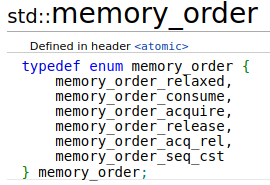
\includegraphics[width=0.8\linewidth]{modes.png}}
    \end{column}
    \begin{column}{0.4\linewidth}
      {\large ARMv8, etc : \sout{$acyclic(\lPO \cup \lRF)$}}
    \end{column}
    
  \end{columns}
  
\end{frame}

% \begin{frame}{Takeaway}
\begin{frame}
  
  % {\large Summary:}
  % \begin{itemize}
  % \item We describe fairness for operational memory models
  % \item And provide an equivalent uniform declarative definition
  % \item Which is used to prove lock algorithms termination.
  % \end{itemize}
  
  \begin{center}
    \spinlockClientIIExpanded
    \vspace{0.5cm}
    terminates because
  \end{center}
  
  \begin{columns}
    \begin{column}{0.4\linewidth}      
      \scalebox{0.5}{\begin{traceenv}{1.4}{0.9}
        \stepcounter{evctr}
        \node at (\curEv-0.5, 1) {$CAS(l, 0, 1)$ \stepcounter{evctr}};
        \node at (\curEv-0.7, 0) {$CAS(l, 0, 1)$ \stepcounter{evctr}};
        \node at (\curEv-0.4, 0) {$CAS(l, 0, 1)$ \stepcounter{evctr}};
        \node at (\curEv-0.7, 1) {$\writeInst{l}{0}$ \stepcounter{evctr}};
        \node at (\curEv-0.7, 0) {\color{red} $CAS(l, 0, 1)$ \stepcounter{evctr}};
        \node at (\curEv-0.8, 1) {\color{blue} \underline{$\mathtt{something \ happens}$} \stepcounter{evctr}};
        
        \node at (\curEv-0.7, 0) {\color{blue} $CAS(l, 0, 1)$ \stepcounter{evctr}};
        \node at (\curEv-0.7, 0) {\color{blue} $\writeInst{l}{0}$ \stepcounter{evctr}};
      \end{traceenv}
      }
    \end{column}    
    \begin{column}{0.4\linewidth}
      \renewcommand{\hof}{2}
      \renewcommand{\vof}{1}
      \scalebox{0.8}{
      \begin{tikzpicture}[xscale=2, yscale=0.8]
        \spinlockContraGraphEventsI
        \spinlockContraGraphRelationsI
        \spinlockContraGraphEventsII
        \spinlockContraGraphRelationsII
      \end{tikzpicture}
      }
    \end{column}
  \end{columns}

  % \todo{{\large More in the paper: ?}}

\end{frame}
%%% Local Variables:
%%% mode: latex
%%% TeX-master: "oopsla"
%%% End:
